\chapter{Further Plots}

\newpage
\section{First Generation Experiments :  Winning Ratio Plots}
\begin{figure}[H]
\centering
    \begin{subfigure}[t]{0.8\textwidth}
    \centering
        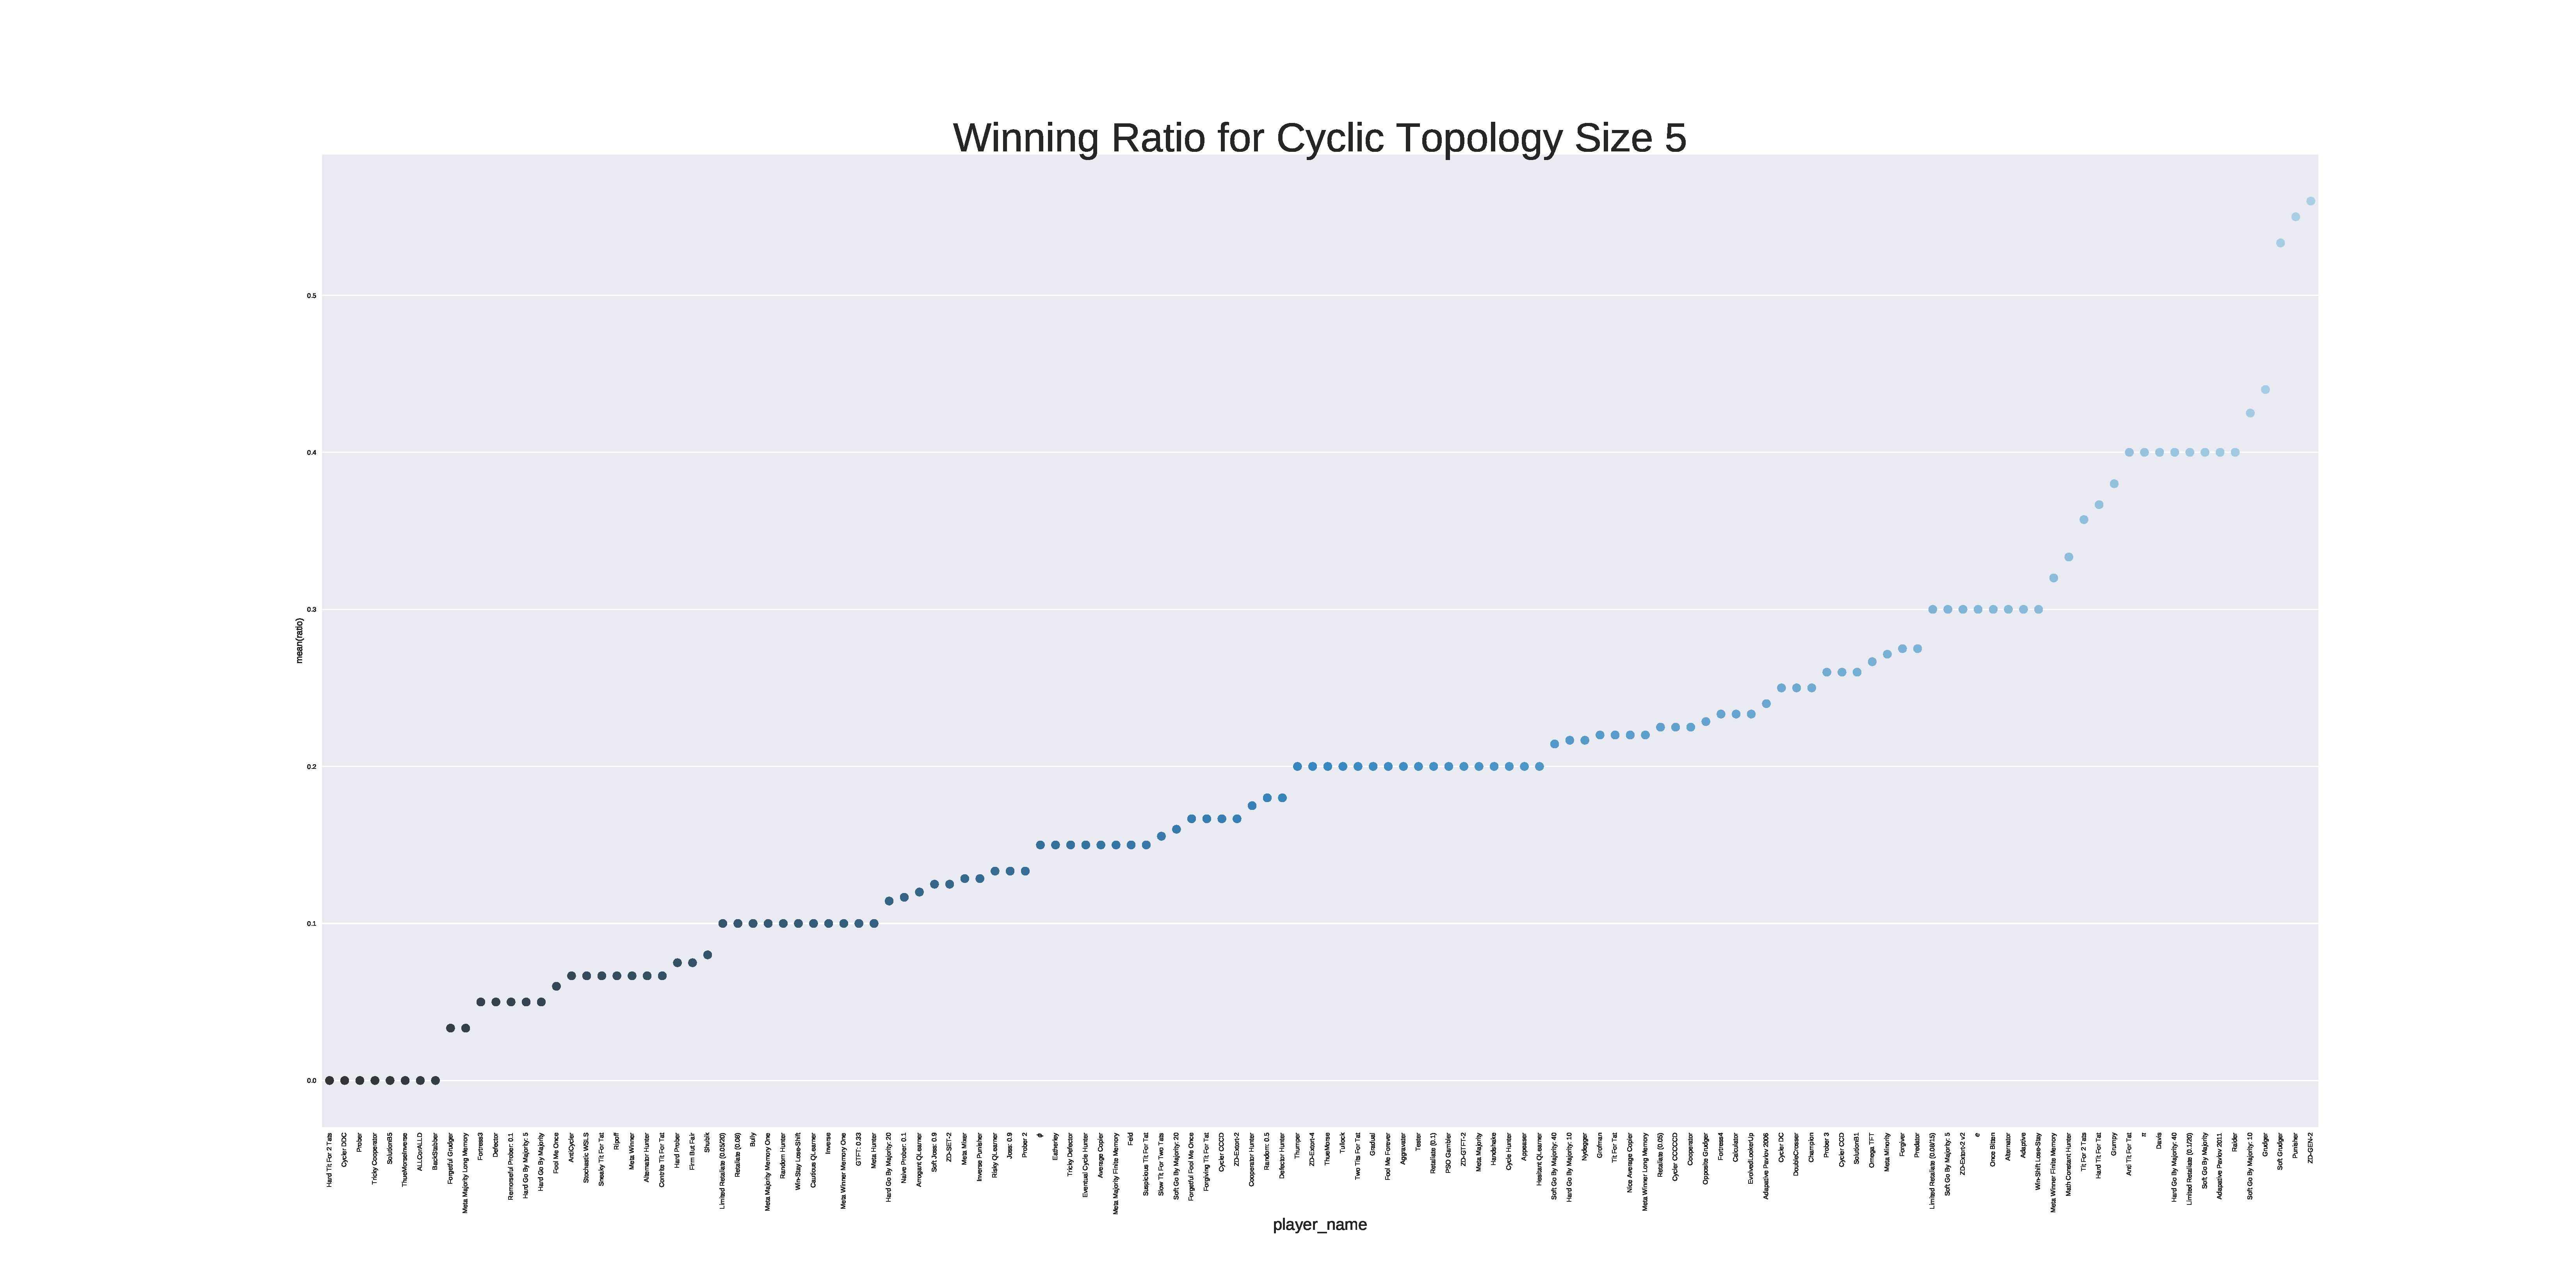
\includegraphics[width=\linewidth]{appendix/winners-Cyclic-5.pdf}
    \caption{Winning ration cycle s=5.}
    \end{subfigure}
\hfill
    \begin{subfigure}[t]{0.8\textwidth}\centering
    \centering
        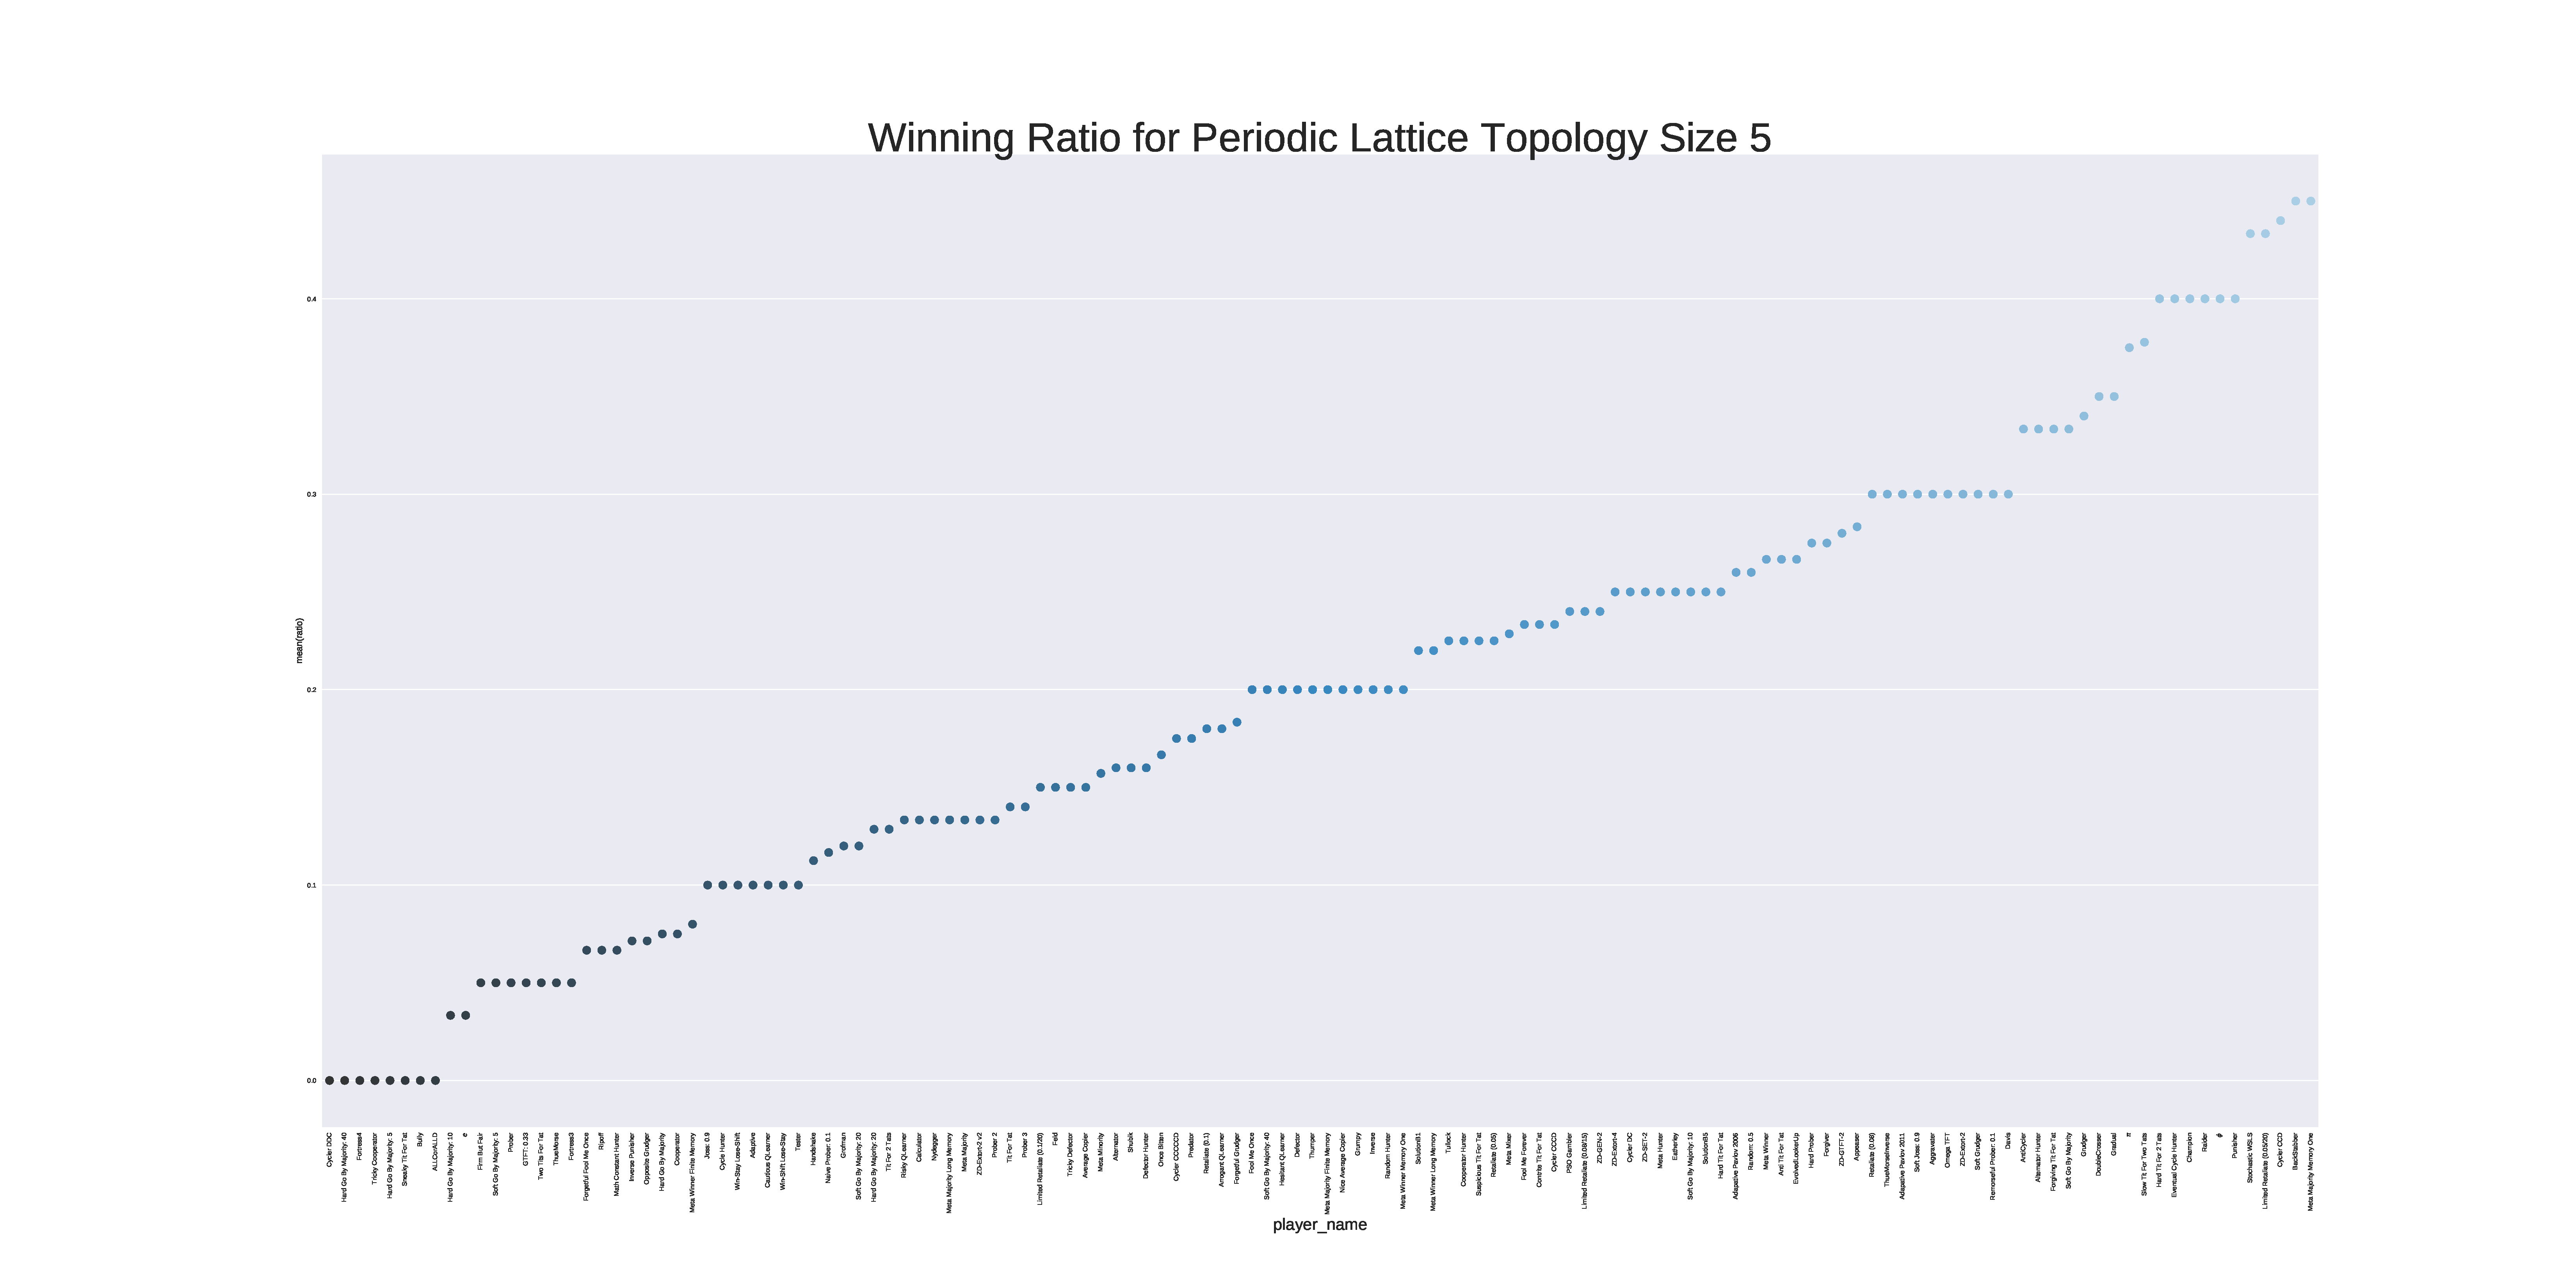
\includegraphics[width=\linewidth]{appendix/winners-Periodic-Lattice-5.pdf}
    \caption{Winning ration lattice s=5.}
    \end{subfigure}
\hfill
    \begin{subfigure}[t]{0.8\textwidth}\centering
    \centering
        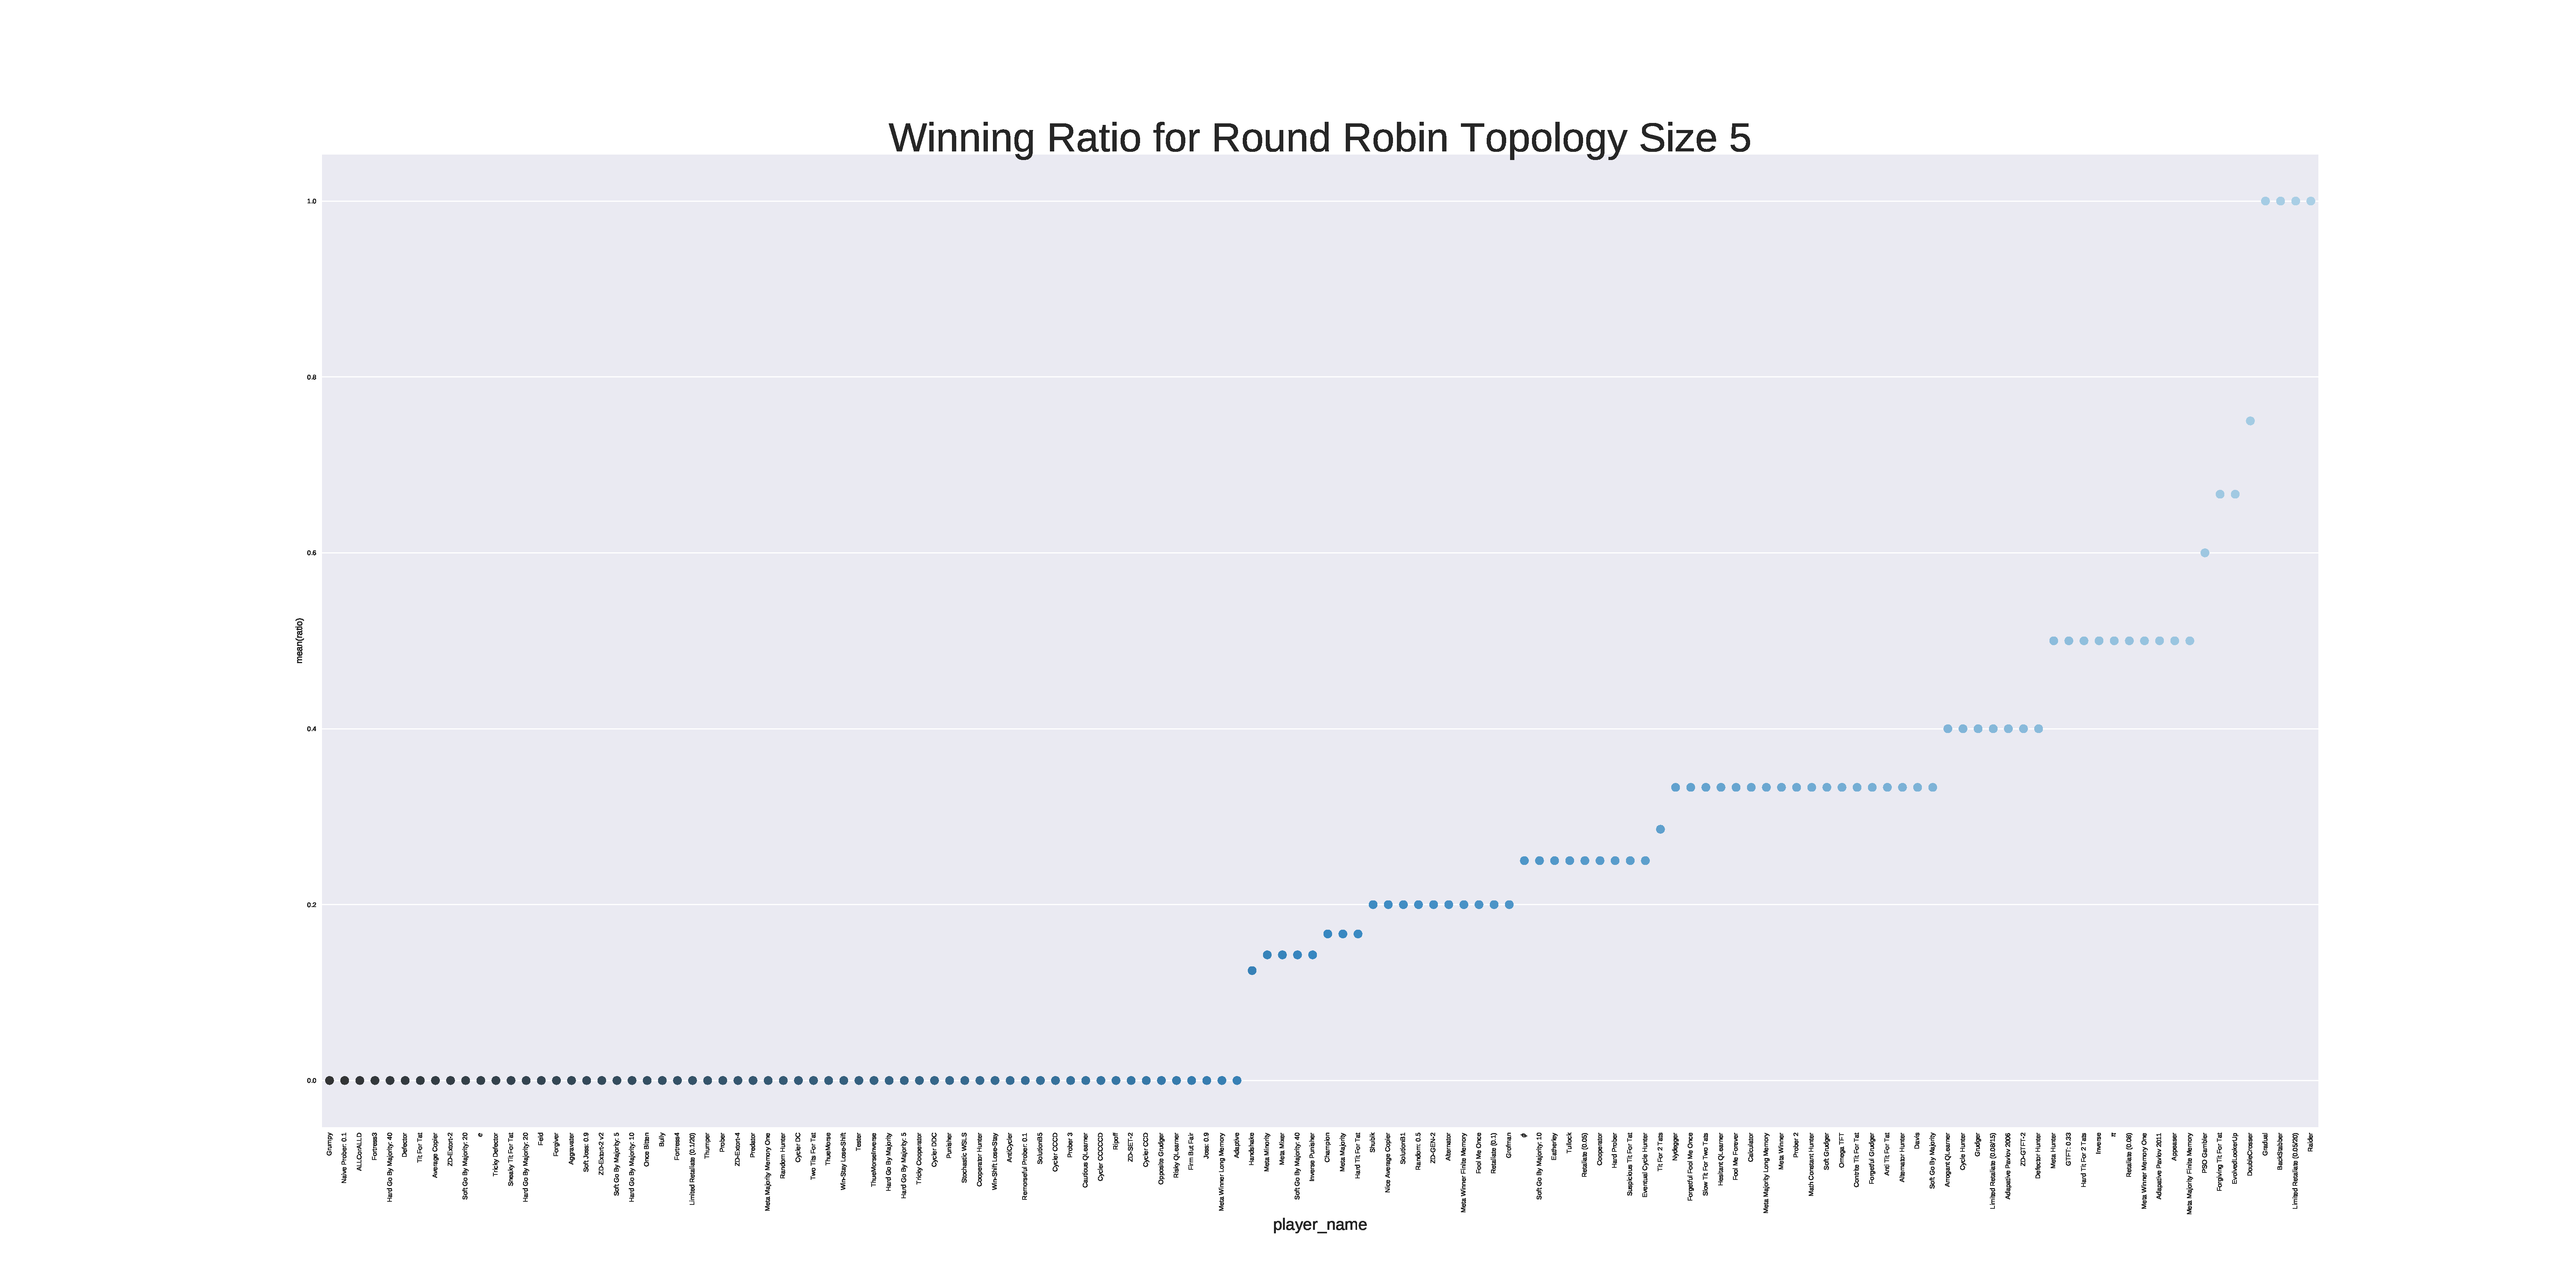
\includegraphics[width=\linewidth]{appendix/winners-Round-Robin-5.pdf}
    \caption{Winning ration round robin s=5.}
    \end{subfigure}
\caption{Winning ratio for all three topologies s=5.}
\label{fig:winning-five}

\end{figure}

\begin{figure}[H]
\centering
    \begin{subfigure}[t]{0.8\textwidth}
    \centering
        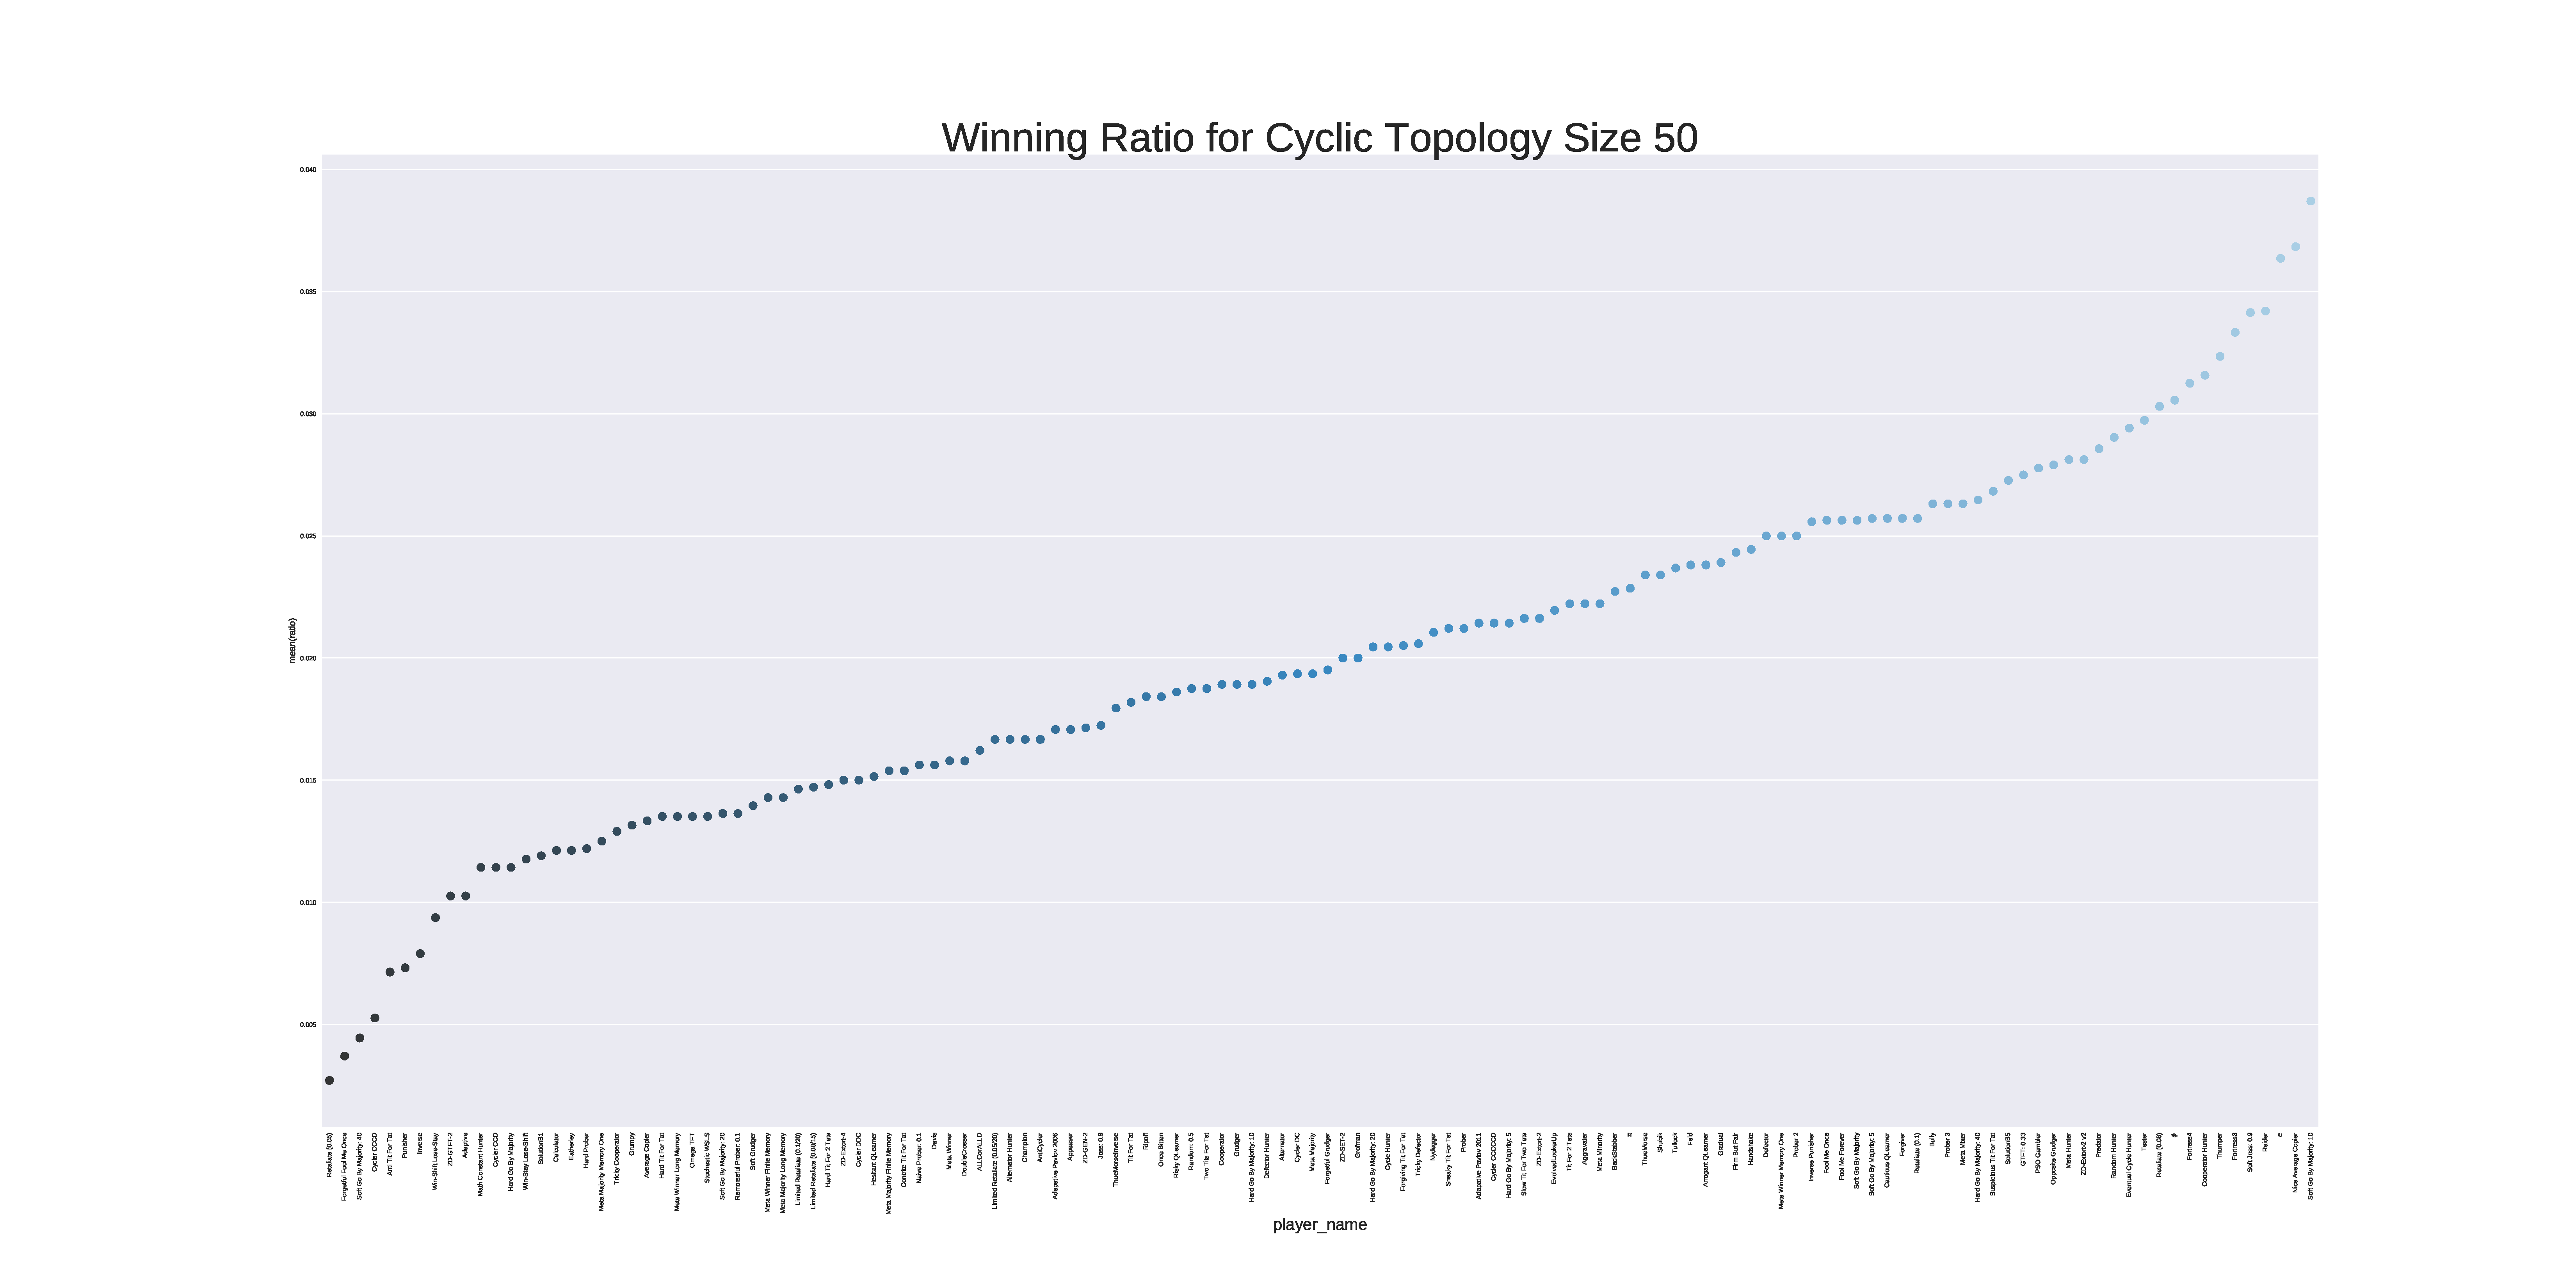
\includegraphics[width=\linewidth]{appendix/winners-Cyclic-50.pdf}
    \caption{Winning ration cyclic s=50.}
    \end{subfigure}
\hfill
    \begin{subfigure}[t]{0.8\textwidth}\centering
    \centering
        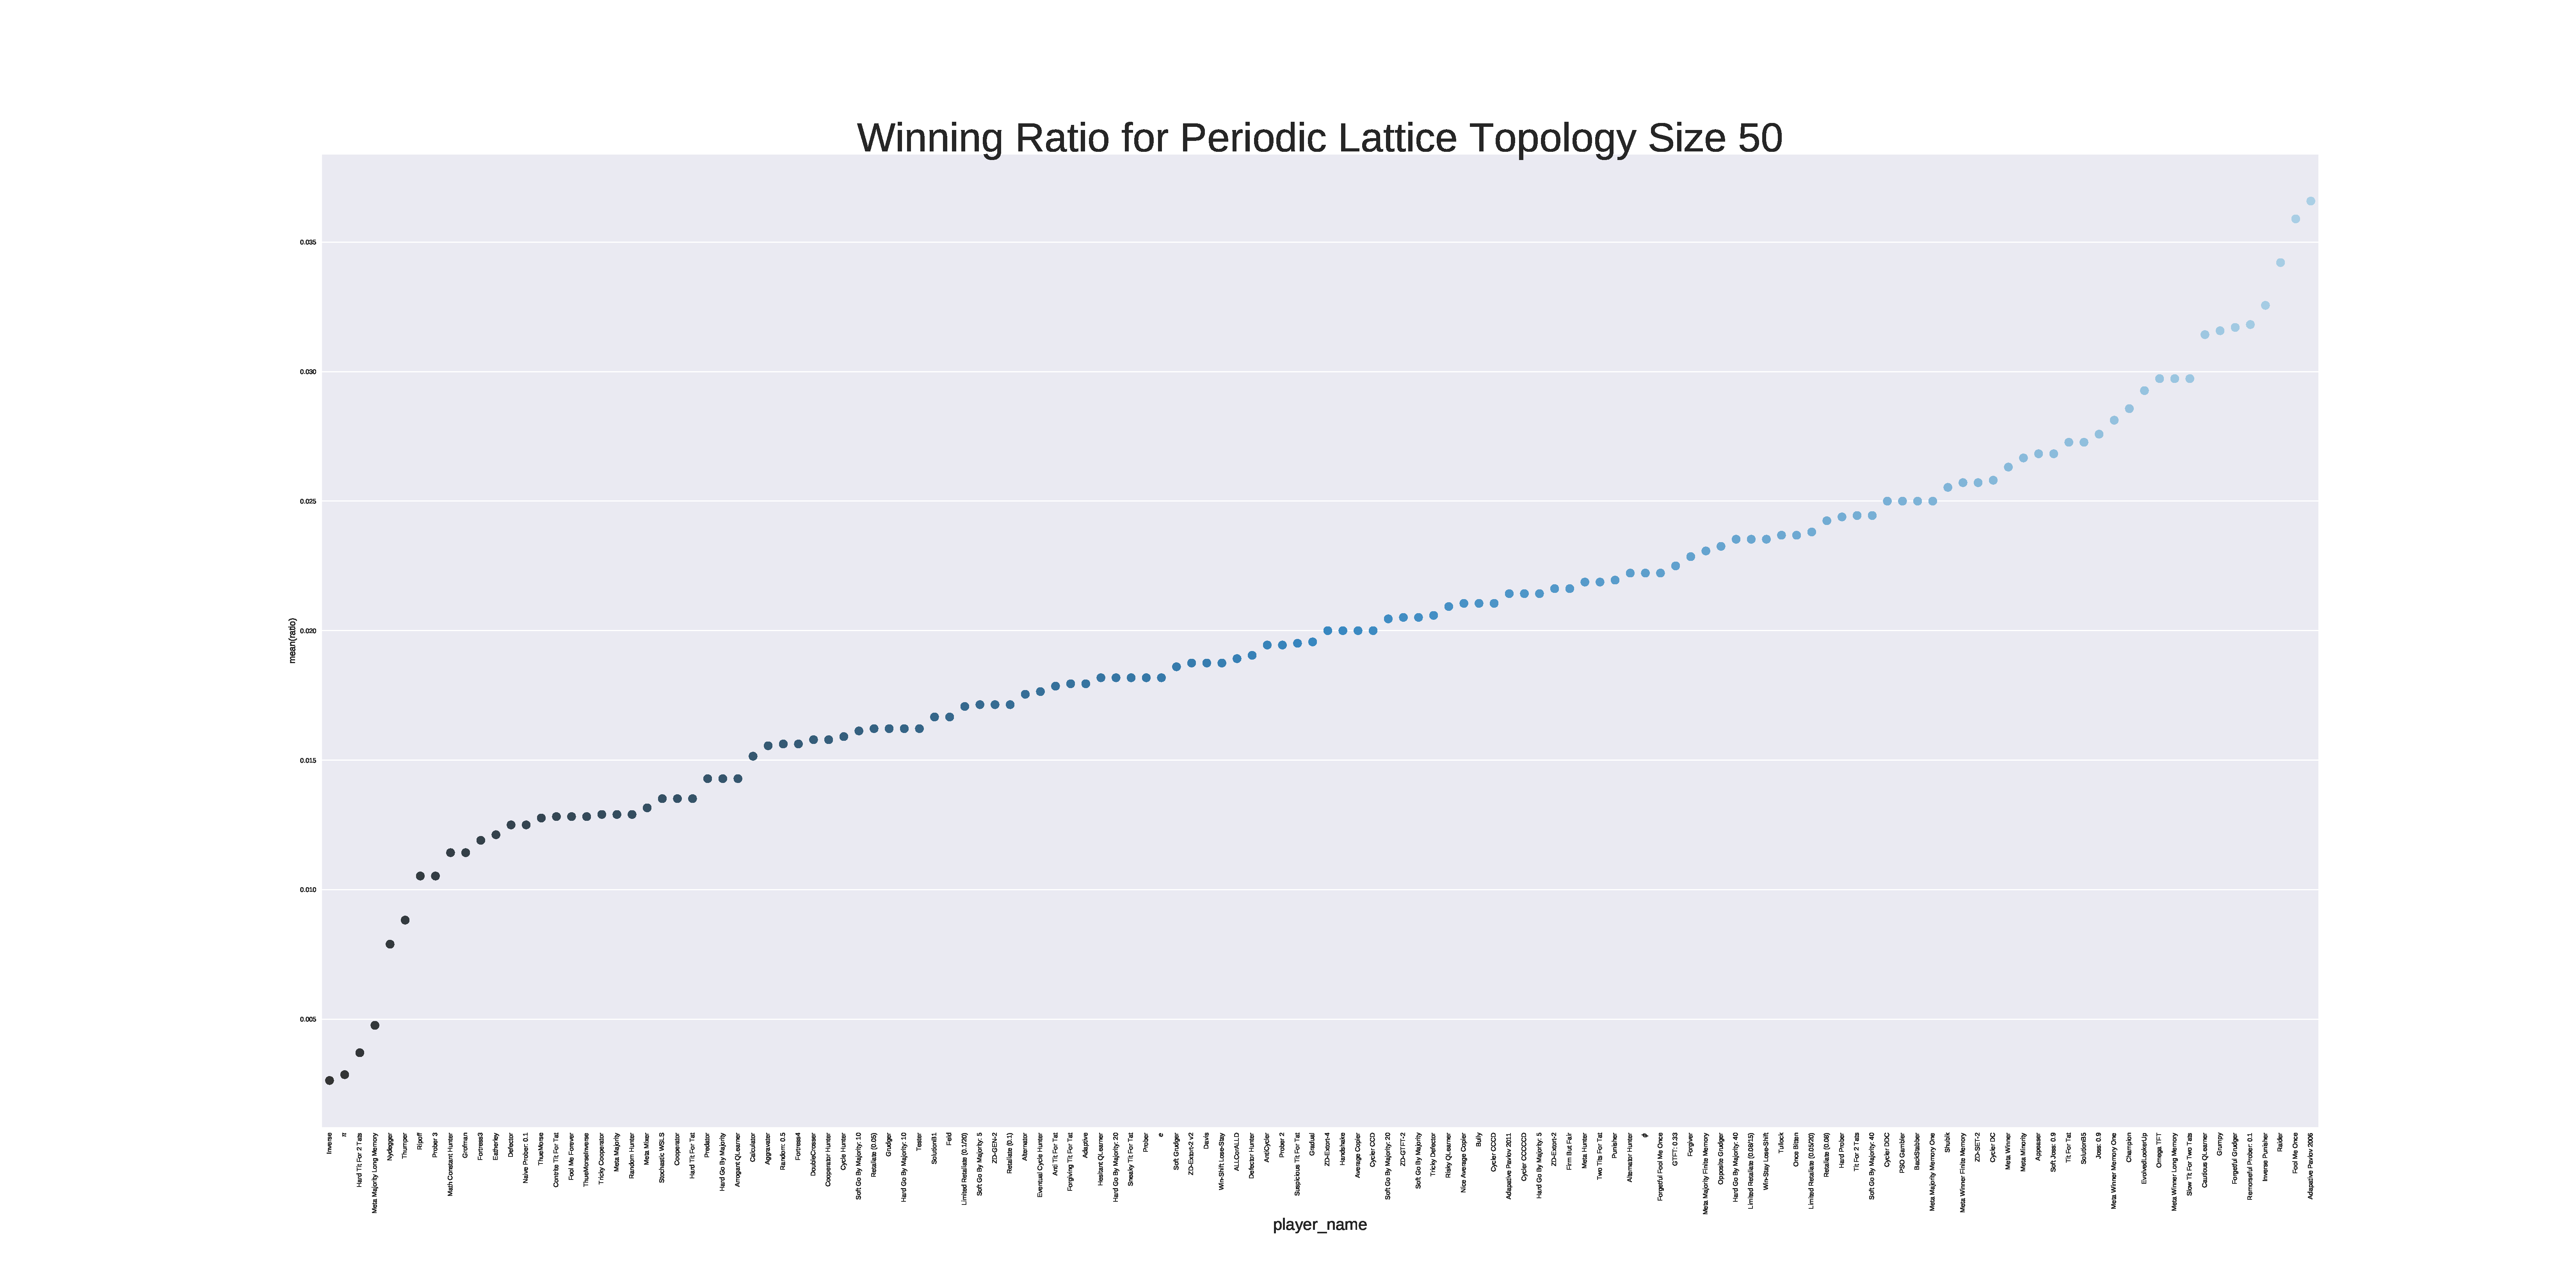
\includegraphics[width=\linewidth]{appendix/winners-Periodic-Lattice-50.pdf}
    \caption{Winning ration lattice s=50.}
    \end{subfigure}
\hfill
    \begin{subfigure}[t]{0.8\textwidth}\centering
    \centering
        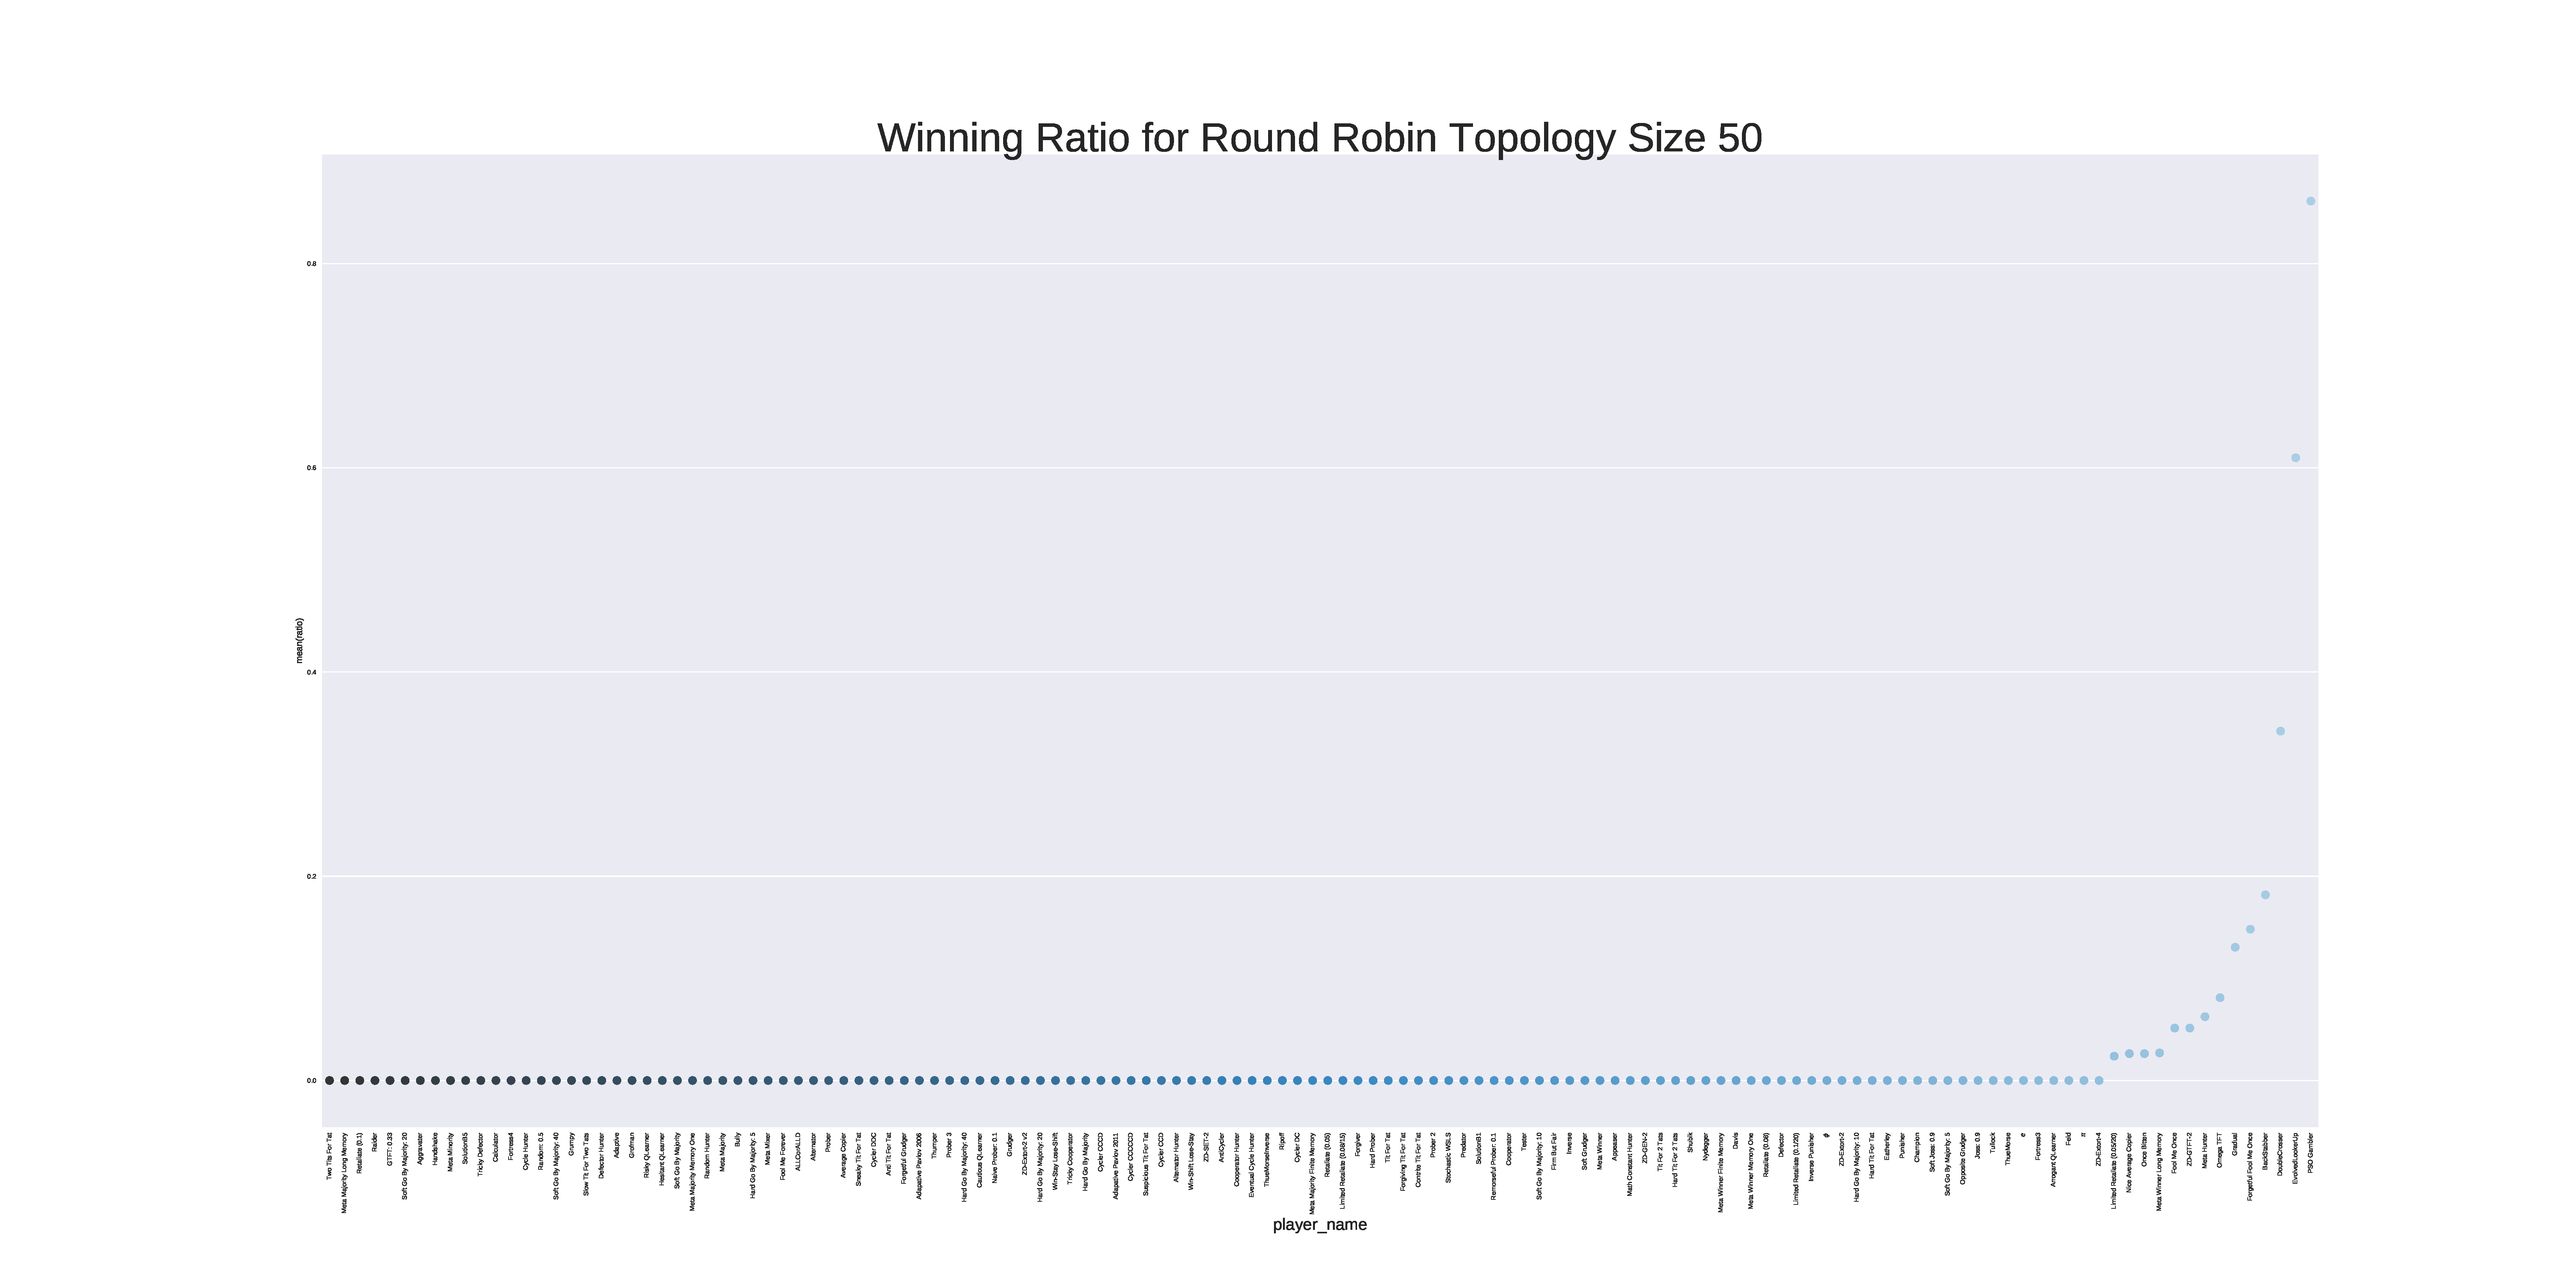
\includegraphics[width=\linewidth]{appendix/winners-Round-Robin-50.pdf}
    \caption{Winning ration round robin s=50.}
    \end{subfigure}
\caption{Winning ratio for all three topologies s=50.}
\label{fig:winning-fifty}
\end{figure}

\chapter{Second Appendix Title}
